\section{Arquitectura de Redundancia Propuesta RE ACOMODAR EN OTRA SECCIÓN}

% En esta sección, se presenta la arquitectura implementada para la tolerancia a fallas de hardware. Como se mostró en la sección anterior, \textit{The Byzantine Generals Problem} sienta las bases para la tolerancia a fallas arbitrarias de hardware. A través de una serie de intercambios de mensajes entre los nodos de la red, estos pueden llegar a un consenso, para tomar la misma decisión. Además, se mostró que para poder tolerar una falla arbitraria, se requiere por lo menos de 4 nodos interconectados.

% Luego de presentar el problema, se hizo una comparación entre los generales leales y las computadoras de vuelo sin fallas y entre los generales traidores y las computadoras con fallas. Una de las cuestiones que no se mencionó, es el hecho de que las computadoras de vuelo constituyen sistemas de tiempo real. Esto es debido a que deben realizar tareas que requieren determinismo temporal. Por ejemplo, cálculo de la ley de control, estimación de la pose, etc... En el problema original, los generales pueden enviar sus mensajes a sus pares en cualquier momento y en cualquier orden.

% Otro de los puntos que caracterizan al problema original, es el hecho de que la comunicación entre los generales es 1 a 1. Debido a esto, los generales traidores pueden entregar información confusa a sus pares para tratar de romper el consenso. Esto es lo que vuelve complejo al problema \cite{lamport2019byzantine} y costosa a su solución \cite{roth2021not}.

% En esta sección se muestra que, si el sistema tiene ciertas características, en particular ser un sistema de tiempo real y contar con un bus común a los nodos para las comunicaciones, luego el problema del consenso se simplifica mucho.

\subsection{Simplificación del Problema de Tolerancia a Fallas Arbitrarias de Hardware}

% En sistemas de tiempo real para aplicaciones \textit{safety-critical}, es común encontrar sistemas distribuidos con comunicación a través de un bus. Por ejemplo en los automóviles, los nodos que se encuentran repartidos por todo el vehículo se comunican a través de redes como CAN\cite{specification1991bosch} o FlexRay\cite{nxpAN12233}. Todos los nodos de la red se encuentran conectados al mismo bus de comunicación, por lo que cuando un nodo envía un mensaje a través del bus, todos los demás nodos reciben el mismo mensaje.

% \begin{figure}[H]
%     \centering
%     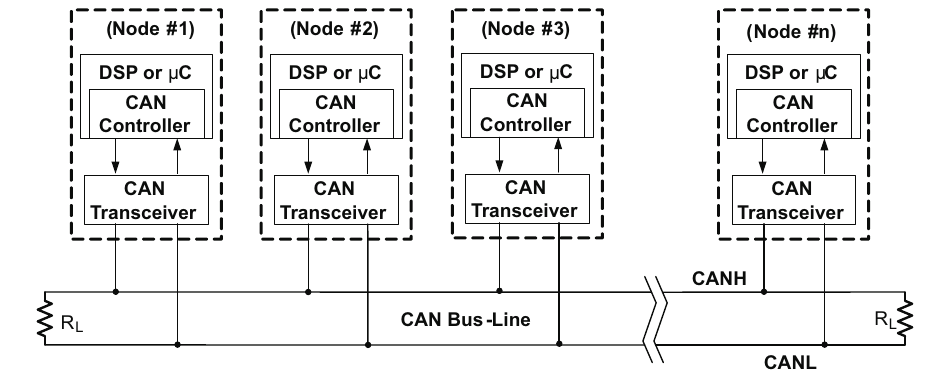
\includegraphics[width=\textwidth]{img/red_CAN.png}
%     \caption{Todos los nodos se encuentran conectados al mismo bus de comunicaciones. En el caso del bus CAN, se compone de dos cables, CAN-H y CAN-L, terminados en sus extremos por resistencias de adaptación. La imagen se extrajo de \cite{texasSLOA101B}.}
%     \label{fig:red_CAN}
% \end{figure}

% Esto presenta una diferencia respecto de lo planteado en \textit{The Byzantine Generals Problem}, ya que la existencia de un bus común a todos los nodos automáticamente elimina la posibilidad de que uno de los miembros de la red pueda enviar información diferente a sus pares. Puede compararse la figura \ref{fig:byzantine_bus_1} con la figura \ref{fig:Byzantine_Generals_Problem_5}.

% \begin{figure}[H]
%     \centering
%     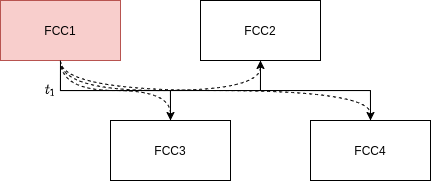
\includegraphics[width=0.6\textwidth]{img/byzantine_bus_1.png}
%     \caption{En este caso, la conexión tipo bus no permite el envío de información diferente a los demás miembros. La FCC1 envía el valor $t_1$ y todos sus pares reciben el mismo valor.}
%     \label{fig:byzantine_bus_1}    
% \end{figure}

% Como contrapartida, debido a que los nodos comparten canal de comunicación, estos deben tomar turnos para enviar la información a sus pares. De otra forma, habría una colisión en el bus y la información nunca llegaría a su destino. Sumado a esto, el bus se convierte en un punto singular de falla, ya que es posible que un problema en el bus deje a los nodos incomunicados.

{\Large \textbf{{\color{red} ACÁ AGREGAR EJEMPLOS DE USO DE DOBLE BUS. POR EJEMPLO LOS AUTOS CON DOBLE CAN O DOBLE FLEX RAY, EL PAPER QUE USA DOBLE TIME TRIGGERED BUS, ETC}}}

% \subsubsection{Consenso}

% Al igual que como se hizo en la sección \ref{sec:consenso_TMR}, se analiza el problema del consenso para la arquitectura propuesta en esta sección. El ejemplo que se presentó anteriormente fue el necesario para lograr una sincronización entre las FCCs y se mostró que el enviar información distinta a cada computadora de vuelo, puede romper el sincronismo muy fácilmente.

% Para el caso en el que se utiliza un bus de comunicación, como se mencionó, las FCCs deben tomar turnos para utilizar el medio físico. En las próximas secciones se explicará cómo se puede lograr esto, aquí se asume que las FCCs respetan sus turnos para utilizar el medio físico compartido. En la figura \ref{fig:byzantine_bus_2}, la FCC1 accede al medio y envía su valor de \textit{timestamp}. Las demás FCCs reciben el mismo valor, por estar conectadas al mismo bus de comunicación. Luego, las FCC2 y 3 repiten esto mismo. En la figura \ref{fig:byzantine_bus_3} se muestra que todas tienen la misma información respecto de sus pares. Luego por ejemplo, si calculan un promedio, llegarán al mismo resultado y se sincronizarán correctamente.

% \begin{figure}[H]
%     \centering
%     \begin{subfigure}[b]{0.34\textwidth}
%         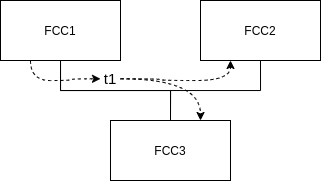
\includegraphics[width=\textwidth]{img/byzantine_bus_2.png}
%         \caption{La FCC1 envía su \textit{timestamp} hacia las demás.}
%         \label{fig:byzantine_bus_2}
%     \end{subfigure}\hfill
%     \begin{subfigure}[b]{0.49\textwidth}
%         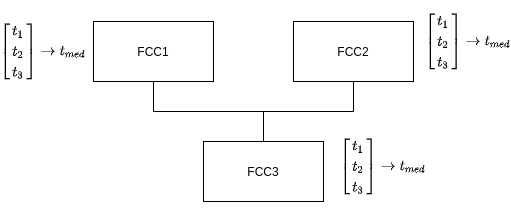
\includegraphics[width=\textwidth]{img/byzantine_bus_3.png}
%         \caption{Luego de finalizar los intercambios, todas las FCCs llegan al mismo resultado de \textit{timestamp} para sincronizarse.}
%         \label{fig:byzantine_bus_3}
%     \end{subfigure}
%     \caption{Debido a la existencia del bus, las FCCs no pueden mentir acerca de su \textit{timestamp}. Luego, todas llegan a un consenso de manera casi trivial.}
%     \label{}
% \end{figure}

% A partir de este análisis, se puede ver que para el caso de un sistema de tiempo real con un único bus de comunicaciones, el problema del consenso es mucho más sencillo que lo que se muestra en \textit{The Byzantine Generals Problem}. De todas maneras, lo que se presenta aquí es un primer análisis, ya que se ha asumido que no hay colisiones en el bus y que los nodos se encuentran sincronizados.

\subsubsection{Sincronismo de los nodos}

En la sección \ref{sec:sincronismo_TMR} se mencionó la necesidad del sincronismo entre los nodos y que esta se logra a partir de un intercambio de mensajes. Para la arquitectura propuesta, ese intercambio de mensajes se hace a través del mismo bus. Debido a que el medio es compartido, los nodos de la red deben tomar turnos para acceder al medio, de manera de que todos puedan enviar sus respectivos mensajes.

Típicamente, una FCC ejecuta las mismas tareas relacionadas al control del vehículo, de manera periódica \cite{hiergeist2018implementation}:

\begin{enumerate}
    \item Lectura de los sensores.
    \item Cálculo de la ley de control.
    \item Aplicación del resultado a los actuadores.
\end{enumerate}

Debido a que se trata de un sistema de tiempo real, cada una de las FCCs debe realizar estas tareas en un período de tiempo dado. En la figura \ref{fig:task_scheduling_1} se muestra un gráfico con la secuencia de ejecución periódica de las tareas.

\begin{figure}[H]
    \centering
    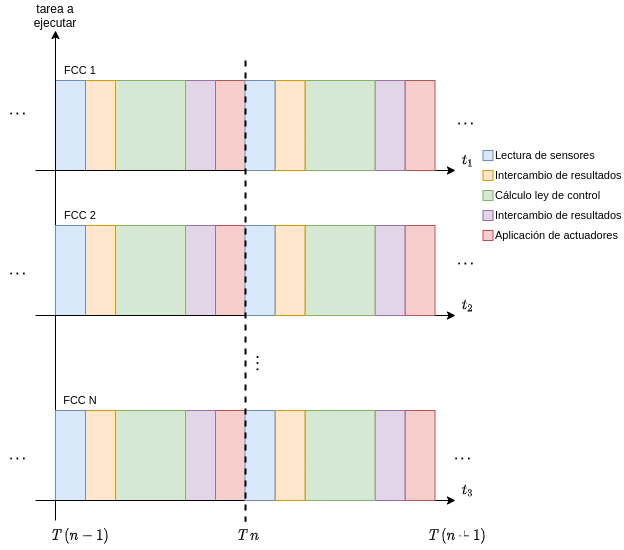
\includegraphics[width=0.7\textwidth]{img/task_scheduling_1.png}
    \caption{El eje horizontal representa el paso del tiempo. Las barras de colores representan el tiempo dedicado a ejecutar cada tarea, como la lectura de sensores, cálculo de la ley de control, etc., de forma periódica. En la imagen se puede ver que las FCC 1, FCC 2, ..., FCC N se encuentran sincronizadas ya que realizan las tareas al mismo tiempo. }
    \label{fig:task_scheduling_1}
\end{figure}

En un sistema con redundancias, como ya se mencionó, cada una de las FCCs realiza las mismas tareas. Además, estas intercambiarán resultados relacionados a mediciones de sensores y a valores de actuación para los motores con sus pares, justamente para enmascarar y tolerar las fallas. A partir de esto, se desprende que el intercambio de mensajes también corresponde a tareas que deben ejecutarse periódicamente y en un determinado período de tiempo acotado.

Cada una de las computadoras de vuelo incluye un clock interno, el cual utiliza como base para cumplir con los tiempos de ejecución. Cuando se habla del sincronismo entre los nodos de la red, lo que se busca es que las ejecuciones de las N computadoras se encuentren coordinadas. Por ejemplo, en la figura \ref{fig:task_scheduling_2} se muestra un caso para dos computadoras de vuelo cuya ejecución se encuentra desfasada. Es fácil ver que este sistema nunca podrá cumplir con el objetivo de controlar el vuelo del UAV.

\begin{figure}[H]
    \centering
    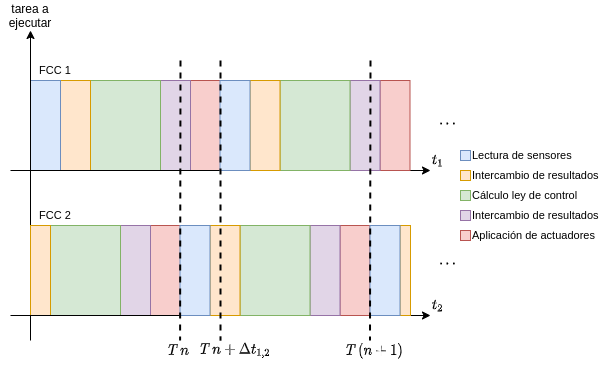
\includegraphics[width=0.7\textwidth]{img/task_scheduling_2.png}
    \caption{Se muestra un ejemplo para dos FCCs. A diferencia de la figura \ref{fig:task_scheduling_1}, las FCC 1 y la FCC 2 se encuentran desincronizadas.}
    \label{fig:task_scheduling_2}
\end{figure}


En la figura, se muestra que cuando la FCC 2 termina de enviar la señal de control a los actuadores (instante $T_n$), la FCC 1 se encuentra intercambiando resultados con la FCC 2. Debido a que la FCC 2 ya pasó dicha tarea, la FCC 1 no recibirá ningún valor de su par y asumirá erróneamente, que la FCC 2 se encuentra en un estado con alguna falla, ya que no responde. Si bien este ejemplo es muy simple, muestra la necesidad de la sincronización entre nodos de la red, siendo el motivo principal, el hecho de que el sistema es de tiempo real.

\subsection{Arquitectura Del Sistema: \textit{The Time-Triggered Architecture}}

A partir de lo analizado hasta aquí, se enumeran los requerimientos más elementales del sistema:

\begin{enumerate}
    \item El sistema es de tiempo real, es decir, se requiere determinismo temporal en la ejecución de las tareas.
    \item El sistema es redundante, por lo que cada nodo ejecuta las mismas tareas en paralelo y al mismo tiempo.
    \item El uso del bus de comunicación obliga al uso de un protocolo de acceso al medio físico compartido (el bus) por turnos, que permita que todos los nodos tengan acceso a este.
\end{enumerate}

A continuación, se presentan distintas arquitecturas posibles para la implementación y se selecciona una de ellas, la \textit{Time-Triggered Architecture}\cite{kopetz2003time}, cuyas características se ajustan a los requerimientos.

{\Large \textbf{{\color{red} ACÁ COMENTAR LAS ALTERNATIVAS DE LAS DISTINTAS ARQUITECTURAS, COMO SUPER LOOP, EVEN TRIGGERED CON RTOS, SIN RTOS Y TIME TRIGGERED. COMENTAR POR QUÉ ELIJO TIME TRIGGERED Y DESCARTO LAS DEMÁS. PONER CASOS DE TRABAJOS CON TTA. EN EL PAPER QUE USA TIME TRIGGERED BUSES HAY VARIOS EJEMPLOS }}}

%\subsubsection{The Time-Triggered Architecture}

En este tipo de arquitectura, el sistema en cuestión ejecuta sus tareas en instantes de tiempo predefinidos. Estas tareas pueden ser tales como tomar datos de un sensor, enviar un dato a otra parte del sistema o realizar algún cálculo. Este tipo de arquitectura es típicamente utilizada en aplicaciones de tiempo real críticas. {\textbf{{\color{red} PONER EJEMPLOS DE SISTEMAS CRÍTICOS CON TIME TRIGGERED ARCHITECTURE}}}. Esto es porque esta arquitectura vuelve al sistema predecible. Teniendo en cuenta lo mencionado en la sección \ref{subsec:introduccion_al_analisis_de_tolerancia_a_fallas}, que el comportamiento del sistema sea predecible lo vuelve más confiable y por ende más seguro.

Existe otro criterio por el cual típicamente se prefiere este tipo de sistemas para aplicaciones de este estilo y tiene que ver con los procesos de validación que deben realizarse frente a entes reguladores. El hecho de tener un sistema cuyo comportamiento es altamente predecible, simplifica mucho su proceso de validación. \textbf{{\color{red} DESARROLLAR ESTA PARTE CON EJEMPLOS Y CITANDO DO-254, ETC}}.

A continuación, se presenta brevemente los componentes y el funcionamiento de la arquitectura para el sistema de este trabajo. Pueden encontrarse trabajos\cite{kopetz2003time}\cite{kopetz1998time} y libros\cite{kopetz-2011} que explican formalmente esta arquitectura y sus distintos componentes con más detalle.

Como ya se mencionó en las secciones anteriores, el sistema se compone de una serie de \textbf{nodos} interconectados a través de un \textbf{bus de comunicación}. Cada uno de los nodos ejecuta una serie de tareas con un \textbf{scheduling} predefinido por el paso del tiempo.

\begin{figure}[H]
    \centering
    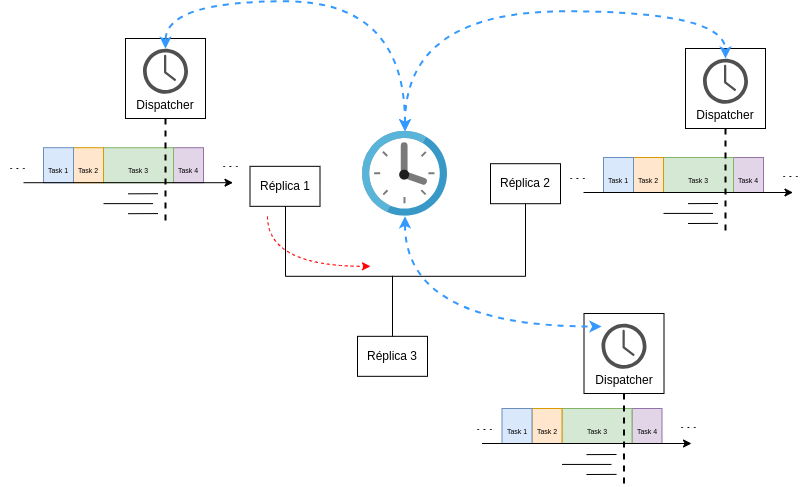
\includegraphics[width=\textwidth]{img/diagrama_TTA.png}
    \caption{Se muestra un esquema que representa la arquitectura. Cada nodo tiene un \textit{clock} local, funcionando a partir de su propio cristal. Todos estos a su vez se sincronizan periódicamente con el \textit{global time}, representado por el reloj azul en el centro. En la imagen, el nodo 1 está enviando un mensaje por el bus. Los demás nodos saben previamente que deben esperar este mensaje.}
    \label{fig:diagrama_TTA}
\end{figure}

Para que el comportamiento de los nodos sea consistente, estos deben estar \textbf{sincronizados}. Se define entonces una base de tiempo global a todos los nodos, denominada en la bibliografía \textbf{global time base}\cite[p.~51]{kopetz-2011}. Esta representa a un reloj que no existe físicamente, sino que es un acuerdo entre los nodos del sistema respecto a un reloj al que todos los nodos deben seguirle el ritmo. Para esto último, cada nodo tiene su propio \textbf{reloj local}.

En la figura \ref{fig:diagrama_TTA} se muestra un esquema de la arquitectura \textit{Time Triggered}. Los tres nodos de la imagen, FCC1, FCC2 y FCC3 se encuentran sincronizados ejecutando la tarea \textit{Task 3}. Esta tarea implica que el nodo FCC1 envíe un mensaje por el bus, representado en la imagen por la flecha roja. En cuanto a los nodos FCC2 y FCC3, la \textit{Task 3} les dice que ellos deben escuchar el bus y esperar el mensaje proveniente del FCC1. Esto quiere decir que el comportamiento predefinido por el scheduler también define en qué instantes de tiempo cada nodo puede enviar un mensaje y en qué instantes de tiempo debe recibirlo. Con respecto a esto último, si en el ejemplo de la figura \ref{fig:diagrama_TTA} el nodo FCC1 presenta una falla y no envía el mesanje en el tiempo correspondiente, luego los nodos FCC2 y FCC3 no recibirán nada. Es común encontrar protocolos de comunicación donde este tipo de fallas se resuelven solicitando el reenvío del mensaje. Sin embargo, debido a que el sistema ya tiene un scheduling predefinido, esto no se permite ya que uno a priori no puede saber si habrá que hacer un pedido de reenvío de mensaje o no, lo que puede corromper el scheduling del sistema. Justamente, la \textit{Time-Triggered Architecture} busca que el sistema sea predecible.

A continuación, se describe brevemente cada uno de los componentes de este tipo de sistema. Para una explicación más detallada, referirse a \cite{kopetz-2011} y \cite{kopetz2003time}.

\subsubsection{Bus de Comunicaciones}

El bus de comunicaciones es el medio a través del cual los nodos intercambian información. Como se describió anteriormente, la arquitectura requiere la sincronización de los nodos para una ejecución consistente. Esto quiere decir que como mínimo, los nodos intercambian mensajes utilizados para la sincronización entre estos. Más allá de esto, en un sistema distribuido, lo más común es que haya un intercambio de información constante entre nodos.

De manera de minimizar las colisiones y favorecer el cumplimiento en el timing del sistema de tiempo real, el envío y recepción de mensajes se implementa por turnos. Esto corresponde a un protocolo de acceso al medio denominado \textit{Time Division Multiple Access} (TDMA). En la figura \ref{fig:TDMA_esquema} se grafica esto para 3 nodos. Este protocolo define en qué instantes de tiempo cada uno de los nodos puede utilizar el medio físico y en cuáles no. Para que no haya colisiones, todos los nodos deben respetar ese timing, el cual se encuentra predefinido. 

\begin{figure}[H]
    \centering
    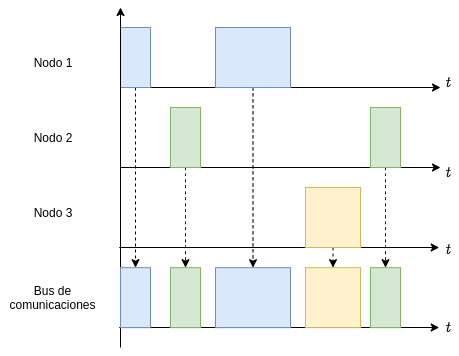
\includegraphics[width=0.7\textwidth]{img/TDMA_esquema.png}
    \caption{El ejemplo muestra como los 3 nodos pueden compartir el bus de comuncaciones. Cada uno de ellos sabe en qué instante de tiempo enviar un mensaje y en qué instantes de tiempo no deben hacerlo y solamente pueden escuchar el bus. Para que esto funcione adecuadamente, los nodos deben estar sincronizados.}
    \label{fig:TDMA_esquema}
\end{figure}

\textbf{{\color{red} ACÁ MENCIONAR ALGUNOS PROTOCOLOS COMO FLEXRAY O TTP/C QUE DE POR SÍ YA EJECUTAN UNA SINCRONIZACIÓN.}}

En \cite{kopetz2003time} se define un elemento del nodo denominado \textit{Communication Network Interface}(CNI). Esta es una interfaz entre el software del nodo y el acceso al medio físico. Utilizando el protocolo de acceso al medio TDMA, el software del nodo \textit{pushea} un mensaje a la CNI. Es esta última la que se encarga de administrar los tiempos de envío y recepción. Es decir, mientras el nodo continua con sus tareas, la CNI se encarga de cumplir con el timing del envío del mensaje.

\begin{figure}[H]
    \centering
    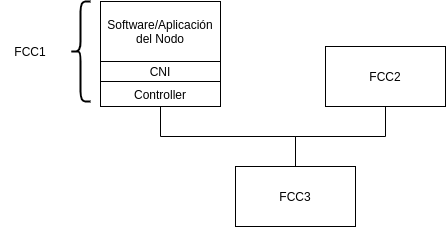
\includegraphics[width=0.6\textwidth]{img/TTA_Bus.png}
    \caption{Misma imagen que \ref{fig:byzantine_bus_2}. Se muestra el detalle de los nodos, en el nodo FCC1.}
    \label{fig:TTA_Bus}
\end{figure}

Al recibir un mensaje, ocurre algo similar. El software del nodo \textit{pollea} a la CNI en determinado instante de tiempo para obtener el mensaje recibido. Otra forma de implementar esto podría ser a través de una interrupción en el software, es decir, que cuando llege un mensaje nuevo, se dispare una interrupción en el software. El problema con esto es que se le quita determinismo al sistema.

\subsubsection{Nodos}

Los nodos son la unidad elemental de los sistemas distribuidos, y también de la arquitectura \textit{Time-Triggered}. Estos son los que ejecutan las tareas y le dan vida al sistema. Los nodos se componen generalmente de un procesador (microcontrolador en el caso de este trabajo), un clock local (en este trabajo se implementa con un circuito oscilador con un cristal) una unidad de control de acceso al bus de comunicaciones y el software local al nodo. En la sección anterior además, se mencionó la existencia de un elemento llamado CNI, que comunica al software con el bus. Sumado a esto, el nodo a su vez contiene un scheduler, el cual se describie en la próxima sección.

\subsubsection{Scheduler}

El sistema conformado por el conjunto de nodos y las comunicaciones entre ellos, se basa en un esquema de tareas que se encuentra predefinido. Esto se diferencia de sistemas de otras características como puede ser alguno con una interfaz con una persona. El caso más cercano puede ser el de un telófono celular, el cual tiene una pantalla que el usuario puede presionar en distintos lugares para abrir una aplicación, enviar un mensaje, etc. Cuando esto ocurre, el celular debe dar una respuesta casi inmediata. Este tipo de sistemas se llaman \textit{Event-Triggered} y son controlados por los eventos que pueden ocurrir. A priori, se asumen eventos asincrónicos, es decir, que pueden ocurrir en cualquier momento y en cualquier orden. A diferencia de esto, en un sistema \textit{Time-Triggered} los eventos no pueden ocurrir en cualquier momento. Mejor dicho, los eventos pueden ocurrir en cualquier momento, pero el sistema solamente prestará atención a esos eventos en un lapso de tiempo predefinido.

En los sistemas operativos de tiempo real se definen una serie de tareas, las cuales utiliza un scheduler que determina cuál es la próxima tarea que corresponde ejecutar. Un sistema \textit{Time-Triggered} también define su comportamiento a través de tareas. La diferencia está en la estrategia utilizada por el scheduler. En el caso de un RTOS es común encontrar schedulers \textit{preemptive} con un sistema de prioridad. En un sistema \textit{Time-Triggered}, los schedulers pueden ser \textit{preemptive} o bien cooperativos. La ventaja de utilizar un scheduler cooperativo es nuevamente el determinismo en la ejecución de las tareas \cite[p.~247]{pont2008patterns}.

\subsubsection{Global Time y Sincronización}

De forma de que el funcionamiento del sistema de tiempo real distribuido sea correcto, todos los nodos deben ejecutar sus tareas de forma consistente. Para ello, sus schedulers deben estar sincronizados. Para el caso de este trabajo, cada una de las FCCs debe encontrarse ejecutando la misma tarea al mismo tiempo. De esta forma pueden ejecutarse los algoritmos de votación para realizar tolerancia a fallas de hardware, como ya se describió anteriormente.

Algunos sistemas distribuidos de tiempo real utilizan un clock maestro, implementado como un nodo de la red al que todos los demás nodos utilizan como referencia. Por ejemplo, la extensión del protocolo automotivo CAN, denominada Time-Triggered CAN (TTCAN) \cite{leen2002ttcan} utiliza esta estrategia. La desventaja de este método es que dicho clock maestro se convierte en un punto singular de falla: si este presenta una falla, habrá un error en la sincronización. 

Otra forma es utilizar una \textit{global time base}\cite[p.~51]{kopetz-2011}. Esta se define como un acuerdo entre los nodos de la red respecto a una base de tiempo a utilizar como referencia. Como ya fue mencionado, cada nodo tiene un reloj interno propio, implementado con un cristal oscilador. Esta base de tiempos global puede implementarse por ejemplo utilizando un contador local. Cada nodo incrementa en uno el valor de esta variable, de forma periódica. Para que los nodos puedan utilizar esta variable como base de tiempos, todos los nodos deben tener el mismo número almacenado en su instancia local de dicha variable, al mismo tiempo.

A priori, puede parecer que el hecho de que el valor del contador sea igual en cada nodo al mismo tiempo sea muy exigente. En la implementación, esto no es posible pero tampoco es necesario. Puede existir cierta precisión en la sincronización que dependiendo del hardware y del algoritmo de sincronización, se obtendrá un mejor o peor resultado.

Luego de ejecutar el algoritmo de sincronización, los clocks de cada nodo quedarán sincronizados con cierta precisión $\Phi$. A medida que pase el tiempo, inevitablemente los clocks de cada nodo comenzarán a desfasarse uno del otro, lo cual incrementará el error. Por consiguiente, la sincronización debe ejecutarse de forma periódica. Esto se grafica en la figura \ref{fig:TTA_resincronizacion}.

\begin{figure}[H]
    \centering
    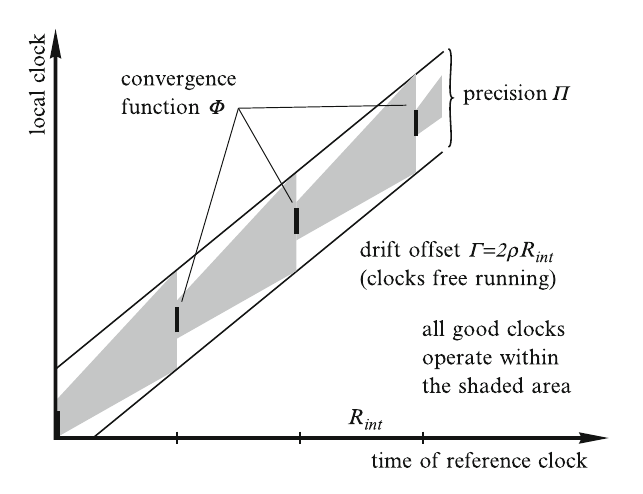
\includegraphics[width=0.7\textwidth]{img/TTA_resincronizacion.png}
    \caption{El eje horizontal representa el paso del tiempo físico y el eje vertical el avance de cada clock local a cada nodo. El valor $R_{int}$ corresponde al período de resincronización. La imagen se extrajo de \cite[p.~67]{kopetz-2011}.}
    \label{fig:TTA_resincronizacion}    
\end{figure}

Existen muchísimos algoritmos de resincronización. En \cite{anceaume1998performance} se puede encontrar un estudio que compara distintos tipos de algoritmos. Un planteo interesante de este trabajo es que los algoritmos de resincronización pueden dividirse en tres bloques básicos, figura \ref{fig:TTA_resincronizacion_building_blocks}, donde lo que varía es la implementación de cada bloque.

\begin{figure}[H]
    \centering
    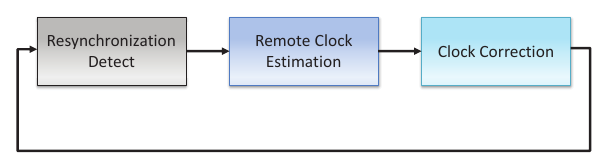
\includegraphics[width=0.8\textwidth]{img/TTA_resincronizacion_building_blocks.png}
    \caption{Tres bloques que comprenden un algoritmo de resincronización. La imagen se extrajo de \cite{de2013overview}.}
    \label{fig:TTA_resincronizacion_building_blocks}
\end{figure}

\begin{enumerate}
    \item \textit{Resynchronization Detect}: Este bloque está dedicado a detectar e informar al nodo de que se va a ejecutar la resincronización.
    \item \textit{Remote Clock Estimation}: Este es el bloque que realiza la cuenta del error entre el clock del nodo y la corrección a aplicar.
    \item \textit{Clock Correction}: Este bloque corresponde a la aplicación de la corrección al clock local.
\end{enumerate}

Para la arquitectura de este trabajo, el primer bloque, \textit{Resynchronization Detect} simplemente consiste en ejecutar una tarea que estará incluida en el scheduling. El segundo bloque es el que realiza el cálculo y puede variar dependiendo de la implementación. Más adelante, se describirá el algoritmo utilizado. Por último, el bloque \textit{Clock Correction}, corresponde a aplicar la corrección al clock local. En general existen dos formas de realizar esto. La primera es pisando el contador existente con el nuevo valor calculado. Este método puede generar inconsistencias en la ejecución de las tareas del nodo \cite[p.~72]{kopetz-2011}. La forma que se prefiere es ir aplicando correcciones sucesivas conforme se van reajustando los clocks. Esto es algo similar a un algoritmo de control, donde se calcula un error y en función de dicho error, se aplica una corrección a la acción de control. En este último caso, la corrección puede implementarse por ejemplo dejando pasar más o menos tiempo para incrementar el contador del clock local.